\باب{بنیادی حقائق}
اس کتاب میں مستعمل حقائق کو اس باب میں اکٹھے کرنے کی کوشش کی گئی ہے۔ توقع کی جاتی ہے کہ یوں کتاب پڑھتے وقت اصل مضمون پر توجہ رکھنا زیادہ آسان ہو گا۔

\حصہ{بنیادی اکائیاں}
اس کتاب میں  \اصطلاح{بین الاقوامی نظامِ اکائی}\حاشیہب{International System Of Units, SI} استعمال کیا گیا ہے جس میں کمیت\حاشیہب{mass} کی اکائی \اصطلاح{کلوگرام}،  لمبائی کی اکائی \اصطلاح{میٹر} اور وقت کی اکائی \اصطلاح{سیکنڈ} ہے۔

\حصہ{غیر سمتی}
وہ متغیر جس کی مقدار (مطلق قیمت) اس کو مکمل طور پر بیان کرتی ہو  \اصطلاح{غیر سمتی}\فرہنگ{غیر سمتی}\حاشیہب{scalar}\فرہنگ{scalar}  متغیر کہلاتا ہے۔ اس کتاب میں غیر سمتی متغیر کو سادہ طرز کی لکھائی میں انگریزی یا لاطینی زبان کے چھوٹے حروف  یعنی \عددی{a,b,\alpha,\cdots}  یا بڑے حروف یعنی  \عددی{A,B,\Psi,\cdots} سے ظاہر کیا جائے گا، مثلاً برقی رو کو \عددی{i} یا \عددی{I} سے ظاہر کیا جاتا ہے۔

\حصہ{سمتیہ}
وہ متغیر جس کو مکمل طور پر بیان کرنے کے لئے اس کی مقدار (طول یا مطلق قیمت) اور سمت جاننا ضروری ہو،  \اصطلاح{سمتیہ}\فرہنگ{سمتیہ}\حاشیہب{vector}\فرہنگ{vector} کہلاتا ہے۔ سمتیہ کو انگریزی یا لاطینی زبان کے چھوٹے یا  بڑے حروف،  جن کو موٹے طرز کی لکھائی میں لکھا گیا ہو،  سے ظاہر کیا جائے گا، مثلاً قوت کو \سمتیہ{F} سے ظاہر کیا جائے گا۔یہاں شکل \حوالہ{شکل_حقائق_اکائی_سمتیہ}  سے رجوع کرنا بہتر ہو گا۔ وہ سمتیہ جس کا طول ایک کے برابر ہو، \اصطلاح{اکائی سمتیہ}\فرہنگ{اکائی سمتیہ}\حاشیہب{unit vector}\فرہنگ{unit vector} کہلائے گا۔ اس کتاب میں اکائی سمتیہ کو انگریزی زبان کے پہلے حرف کو موٹے طرز کی لکھائی میں لکھا جائے گا، مثلاً اکائی سمتیہ \عددیء{\ax,\ay,\az} خلاء کی تین عمودی سمتیات  کو ظاہر کرتے ہیں۔\عددیء{\ax} لکھتے ہوئے، زیر نوشت میں \عددیء{x}، اس بات کی نشاندہی  کرتا ہے کہ یہ اکائی سمتیہ خلاء کی \عددیء{x} سمت کو ظاہر کرتا ہے۔ اگر کسی سمتیہ  کا طول اور اس کی سمت کو علیحدہ علیحدہ لکھنا ہو تو اس کے طول کو ظاہر کرنے کے لئے سادہ طرز کی لکھائی میں وہی حرف استعمال کیا جائے گا جو اس سمتیہ کو ظاہر کرنے کے لئے، موٹے طرز کی لکھائی میں، استعمال کیا گیا ہو۔ یعنی سمتیہ \سمتیہ{F} کے طول کو \عددیء{F} سے ظاہر کیا جائے گا۔ شکل میں سمتیہ  \سمتیہ{F} کا طول \عددیء{F}، چار کے برابر ہے۔ اگر کسی سمتیہ کی سمت میں ایک اکائی سمتیہ بنایا جائے تو یہ اکائی سمتیہ اس سمتیہ کی سمت کو ظاہر کرتا ہے۔جیسے پہلے ذکر ہوا ہے  ایسے اکائی سمتیہ کو انگریزی کے پہلے حرف،  جس کو موٹے طرز کی لکھائی میں لکھا گیا ہو  سے ظاہر کیا جائے گا یعنی سمتیہ \سمتیہ{F} کی سمت کو \عددیء{\سمتیہ{a}_F} سے ظاہر کیا جائے گا۔یہاں،  زیر نوشت میں \عددیء{F} ، اس بات کی یاد دہانی کراتا ہے کہ یہ اکائی سمتیہ \سمتیہ{F} کی سمت کو ظاہر کرتا ہے۔ شکل \حوالہ{شکل_حقائق_اکائی_سمتیہ} میں قوت \سمتیہ{F} کا رخ دائیں  ہے لہٰذا  \عددیء{\سمتیہ{a}_F} اور  \عددیء{\ax} برابر ہوں گے۔
\begin{figure}
\centering
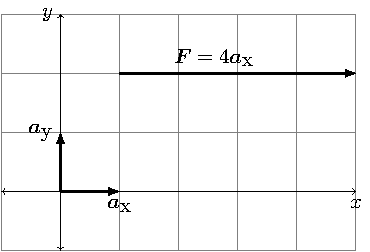
\includegraphics{figBasicFactsUnitVectors}
\caption{کارتیسی محدد}
\label{شکل_حقائق_اکائی_سمتیہ}
\end{figure}
%
\حصہ{محدد}
ایسا طریقہ جس کے ذریعہ کسی نقطہ کا مقام متعین کیا جا سکے محدد کہلاتا ہے۔

خلاء  تین بعدی (تین طرفہ) \حاشیہب{three dimensional} ہے لہٰذا  کسی ایک نقطہ کے مقام کو تین محدد کی مدد سے ظاہر کیا جا سکتا ہے۔اسی طرح  خلاء میں سمتیہ کو تین عمودی اکائی سمتیوں کی مدد سے لکھا جا سکتا ہے۔اب ہم ایسے چند محدد کے نظام دیکھتے ہیں۔

\جزوحصہ{کارتیسی محددی نظام}
شکل \حوالہ{شکل_حقائق_اکائی_سمتیہ}   میں خلاء کی دو سمتوں کو  اکائی سمتیات \عددیء{\ax} اور \عددیء{\ay} سے ظاہر کیا گیا ہے جو آپس میں عمودی ہیں، یعنی، ان کے بیچ \عددیء{90\degree}  زاویہ ہے۔خلاء تین بعدی ہے لہٰذا اسے تین آپس میں \اصطلاح{عمودی اکائی سمتیات}\فرہنگ{سمتیہ!عمودی اکائی}\حاشیہب{orthonormal vectors}\فرہنگ{orthonormal} سے ظاہر کیا جاتا ہے۔ ان سمتوں کے رخ،  طول (لمبائیوں)  کو \عددیء{x,y,z} سے ظاہر کیا جاتا ہے۔ آپ ان سے بخوبی واقف ہیں۔ 

 دائیں ہاتھ کا انگوٹھا، شہادت کی انگلی اور  بڑی انگلی کو ایک دوسرے کے ساتھ \عددی{90^{\circ}} زاویہ پر رکھتے ہوئے اگر شہادت کی انگلی \عددی{\ax} اور بڑی انگلی \عددی{\ay} کے رخ ہوں تب انگوٹھا \عددی{\az} کے رخ ہو گا (شکل \حوالہ{شکل_حقائق_دائیں_ہاتھ})۔ اسی لئے  تین اکائی سمتیات کا یہ نظام \اصطلاح{دائیں ہاتھ کا نظام}\حاشیہب{right handed coordinate system}  کہلاتا ہے۔

\begin{figure}
\centering
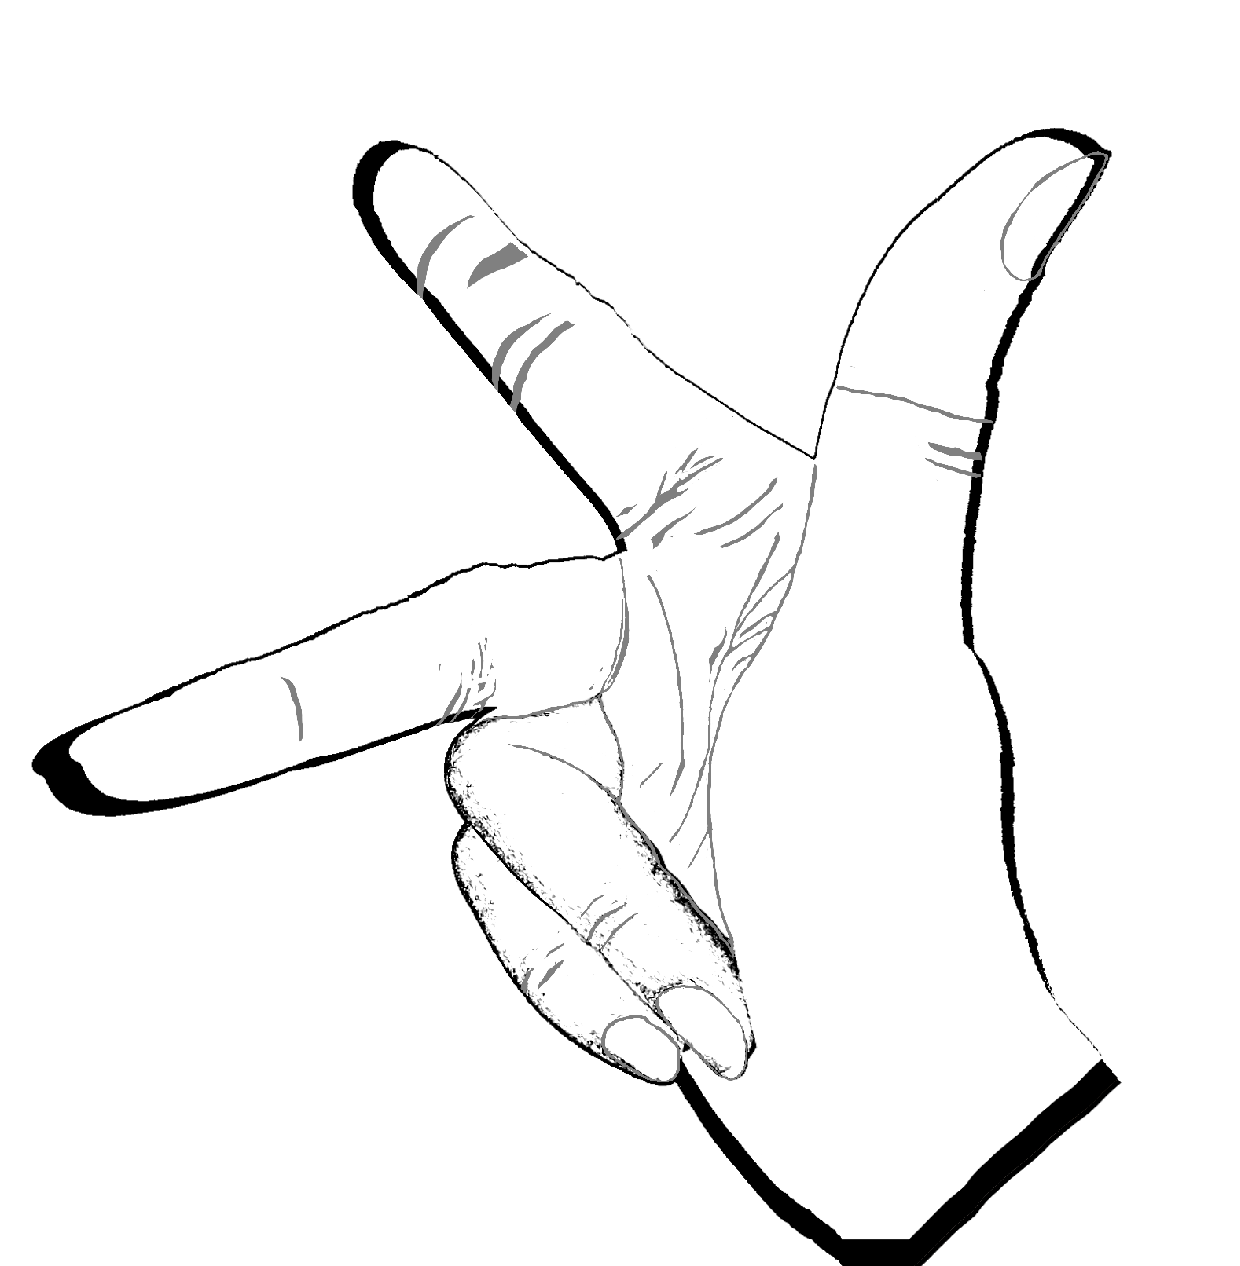
\includegraphics[height=3.5cm]{figRightHandRule}
\caption{دائیں ہاتھ کا نظام۔}
\label{شکل_حقائق_دائیں_ہاتھ}
\end{figure}
مبدا سے نقطہ \عددی{P(x,y,z)} تک سمتیہ \سمتیہ{A} کو شکل \حوالہ{شکل_حقائق_کارتیسی_نظام_ایک_سمتیہ} میں دکھایا  گیا ہے جس کو \اصطلاح{کارتیسی محدد}\فرہنگ{محدد!کارتیسی}\فرہنگ{cartesian system}\حاشیہب{cartesian coordinates} میں تین سمتیات کی مدد سے
\begin{align}
\kvec{A}=\kvec{A}_x+\kvec{A}_y+\kvec{A}_z
\end{align}
یا
\begin{align}
\kvec{A}=x\ax+y\ay+z\az
\end{align}
لکھا جا سکتا ہے۔
%
\begin{figure}
\centering
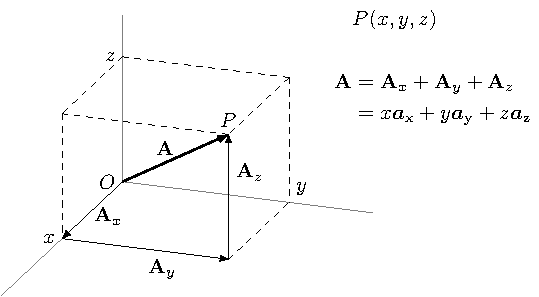
\includegraphics{figBasicFactsVectorCartesianCoordinates}
\caption{کارتیسی محدد نظام میں ایک سمتیہ۔}
\label{شکل_حقائق_کارتیسی_نظام_ایک_سمتیہ}
\end{figure}

کارتیسی محددی نظام میں متغیر \عددی{z}  صفر رکھتے ہوئے \عددیء{x,y} تبدیل کرنے سے  سطح \عددی{xy} ملتی ہے۔ یوں  شکل \حوالہ{شکل_حقائق_کارتیسی_نظام_ایک_سمتیہ}  میں \عددی{P(2,4,3)} لے کر، سطح \عددیء{xy} کو زمین تصور کرتے  ہوئے،  ڈبے کی بالائی سطح پر   \عددیء{z=3} جبکہ \عددی{x} کی قیمت صفر تا  تین اور \عددی{y} کی قیمت صفر تا چار ہو گی۔ اس طرح اس ڈبے کی بالائی سطح درج ذیل لکھی جائے گی۔
\begin{align}
 \text{\RL{ڈبے کی بالائی سطح}}= 
\begin{cases}
    0<x<2\\
    0<y<4 \\
	 z=3
  \end{cases}
\end{align}

متغیر \عددیء{z} کو صفر اور تین کے درمیان ہر ممکن قیمت پر رکھ کر \عددی{x} کو صفر اور دو جبکہ \عددی{y} کو صفر اور چار کے درمیان تبدیل کرنے سے شکل \حوالہ{شکل_حقائق_کارتیسی_نظام_ایک_سمتیہ} میں دکھائے گئے ڈبے کا حجم حاصل ہو گا، لہٰذا اس ڈبے کا حجم درج ذیل لکھا جائے گا۔
\begin{align}
 \text{\RL{ڈبے کا حجم}}=
\begin{cases}
    0<x<2\\
    0<y<4 \\
    0<z<3
  \end{cases}
\end{align}

\جزوحصہ{نلکی محددی نظام}
مبدا سے نقطہ \عددیء{P(x,y,z)} تک  سمتیہ  \سمتیہ{A} کو شکل \حوالہ{شکل_حقائق_نلکی_نظام_ایک_سمتیہ}  میں دکھایا گیا ہے جس  کو دو سمتیات کی مدد سے
\begin{align}
\kvec{A}=\kvec{\rho}+\kvec{A}_z
\end{align}
یا
\begin{align}
\kvec{A}=\rho \arho+z \az
\end{align}
لکھا جا سکتا ہے۔
%
\begin{figure}
\centering
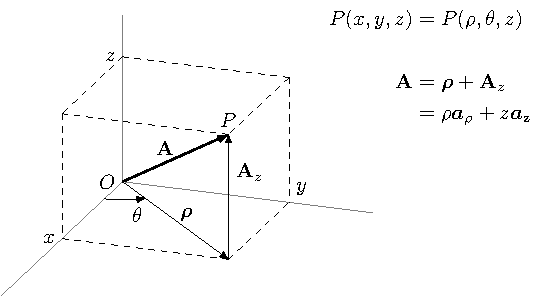
\includegraphics{figBasicFactsVectorCylindricalCoordinates}
\caption{نلکی محددی نظام}
\label{شکل_حقائق_نلکی_نظام_ایک_سمتیہ}
\end{figure}
سمتیہ $\arho$ سطح \عددی{xy} میں پایا جاتا ہے۔ شکل \حوالہ{شکل_حقائق_نلکی_نظام_ایک_سمتیہ} کو دیکھتے ہوئے
\begin{align*}
x=\rho \cos \theta,\quad y=\rho \sin \theta
\end{align*}
لکھ کر نقطہ \عددی{P(x,y,z)} کو متغیرات \عددیء{x,y,z} کے بجائے متغیرات \عددیء{\rho,\theta,z} کی مدد سے \عددیء{P(\rho,\theta,z)} لکھا جا سکتا ہے۔ یوں خلاء میں کسی بھی نقطہ کو اس کے تین متغیرات \عددیء{\rho,\theta,z} سے ظاہر کیا جا سکتا ہے۔

وہ نظام جس میں متغیرات \عددیء{\rho,\theta,z}  کسی نقطہ کو متعین کرتے  ہوں  \اصطلاح{نلکی محدد}\فرہنگ{محدد!نلکی}\حاشیہب{cylindrical coordinates}\فرہنگ{cylindrical coordinates} کہلاتا ہے۔یہاں شکل \حوالہ{شکل_حقائق_نلکی_نظام_تعریف}  سے رجوع کریں۔ نلکی محددی نظام کے تین آپس میں عمودی  اکائی سمتیات $\arho,\atheta,\az$ ہیں۔ یہ نظام بھی دائیں ہاتھ کا نظام ہے لہٰذا دائیں ہاتھ کا انگوٹھا، شہادت کی انگلی اور  بڑی انگلی کو ایک دوسرے کے ساتھ \عددی{90^{\circ}} پر رکھتے ہوئے اگر  شہادت کی انگلی \عددی{\arho} اور بڑی انگلی \عددی{\atheta} کے رخ ہوں تب انگوٹھا \عددی{\az} کے رخ ہو گا۔ 

سطح \عددی{xy} میں مبدا پر، محدد \عددی{x} کے ساتھ  \عددی{\theta} زاویہ پر اکائی سمتیہ  $\arho$ ہو گا۔  سطح  \عددیء{xy} میں مبدا پر اکائی سمتیہ $\arho$ کے عمودی، بڑھتے  \عددی{\theta} رخ، اکائی   سمتیہ $\atheta$ ہو گا۔ کارتیسی محددی نظام کا اکائی سمتتیہ $\az$ ہی نلکی محدد کا اکائی سمتیہ $\az$ ہے۔ 
\begin{figure}
\centering
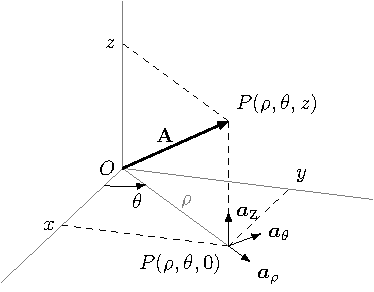
\includegraphics[height=3.5cm]{figBasicFactsCylindricalCoordinates}
\caption{نلکی نما محدد کی تعریف}
\label{شکل_حقائق_نلکی_نظام_تعریف}
\end{figure}

واضح رہے کہ  نلکی محدد کے نظام  میں $\arho$ اور  $\atheta$ کی سمتیں ہر نقطہ پر مختلف ہیں جیسا کہ شکل \حوالہ{شکل_حقائق_نلکی_نظام_میں_اکائی_سمتیات_اٹل_نہیں} میں دکھایا گیا ہے۔
\begin{figure}
\centering
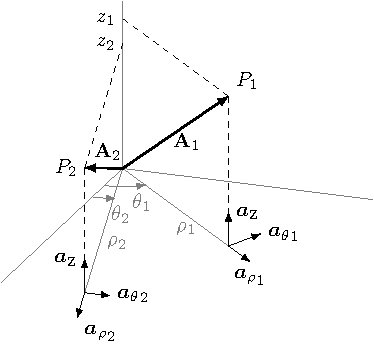
\includegraphics[height=3.5cm]{figBasicFactsCylindricalCoordinatesVaryingUnitVectors}
\caption{نلکی محدد میں اکائی سمتیات \عددیء{\arho} اور \عددیء{\atheta} ہر نقطہ پر مختلف ہیں۔}
\label{شکل_حقائق_نلکی_نظام_میں_اکائی_سمتیات_اٹل_نہیں}
\end{figure}

مستوی \عددی{xy} میں (یعنی \عددی{z=0} لیتے ہوئے) مبدا پر مستقل رداس \عددی{\rho=\rho_0}   کے سمتیہ کو صفر زاویہ پر رکھ کر زاویہ  بتدریج \عددی{2\pi} تک بڑھانے سے سمتیہ کی چونچ مستوی \عددی{xy} میں ایک دائرہ پر چلتی ہے (شکل \حوالہ{شکل_حقائق_نلکی_نظام_میں_دائرہ_اور_نلکی})۔ اب اس سمتیہ کے متغیر \عددی{z} کو تبدیل کرنے سے، مثلاً ہر \عددی{\theta} پر \عددیء{z} کو صفر تا تین کرنے سے، یہ سمتیہ ایک نلکی بنائے گی۔ اسی وجہ سے اس نظام کو نلکی محدد کہتے ہیں۔ سمتیہ کے تینوں متغیرہ تبدیل کرنے سے   نلکی کا حجم ملے گا۔ اگلی تین مساوات ان حقائق کو پیش کرتی ہیں۔
\begin{align}
 \text{دائرہ}&=\begin{cases} 
    \rho=\rho_0\\
    0<\theta<2 \pi \\
    z=0 
\end{cases}\\
 \text{\RL{نلکی نما سطح}}&= \begin{cases}
    \rho=\rho_0\\
    0<\theta<2 \pi \\
  0<z<z_0
  \end{cases}\\
 \text{\RL{نلکی کا حجم}}&= \begin{cases}
    0<\rho<\rho_0\\
    0<\theta<2 \pi \\
  0<z<z_0
  \end{cases}
\end{align}
%
\begin{figure}
\centering
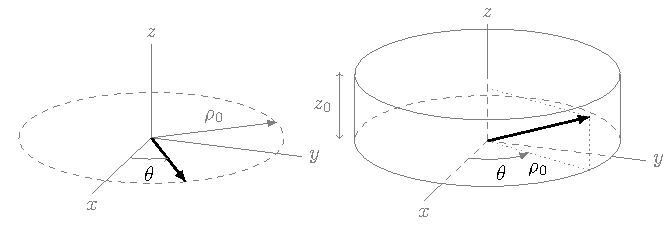
\includegraphics[height=2.5cm]{figBasicFactsCylindricalCoordinatesCircleAndCylinder}
\caption{‫نلکی محدد میں دائرہ اور نلکی‬}
\label{شکل_حقائق_نلکی_نظام_میں_دائرہ_اور_نلکی}
\end{figure}

\حصہ{سمتیہ رقبہ}
سطح پر کھڑا  اکائی سمتیہ سطح کا رخ دیتا ہے (شکل \حوالہ{شکل_حقائق_رقبہ_سمتیہ})۔  چونکہ کسی بھی سطح  کے دو اطراف ہوتے ہیں لہٰذا اس کے دو مخالف  رخ بیان کیے جا سکتے ہیں۔عموماً مسئلہ کو مدِ نظر رکھتے ہوئے  ان میں سے ایک رخ  کو سطح کا رخ  تصور کیا جاتا ہے۔ البتہ بند سطح، مثلاً  گیند، کے بیرونی رخ کو ہی سطح کا رخ تصور کیا جاتا ہے۔شکل \حوالہ{شکل_حقائق_رقبہ_سمتیہ} میں بالائی  سطح \سمتیہ{A_1}  کا رقبہ \عددیء{A_1} ہے اور اس کا رخ $\az$ ہے لہٰذا  \سمتیہ{A_1} سمتیہ کا طول  \عددیء{A_1}  اور رخ $\az$ ہو گا:
\begin{figure}
\centering
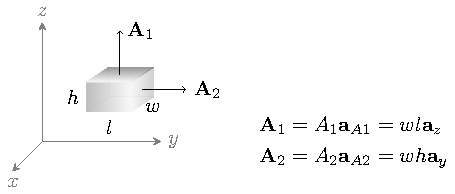
\includegraphics[height=2.5cm]{figBasicFactsVectorArea}
\caption{سمتیہ رقبہ کا تعارف‬}
\label{شکل_حقائق_رقبہ_سمتیہ}
\end{figure}
%
\begin{align*}
A_1&=wl\\
\kvec{a_{A1}}&=\az
\end{align*}
یوں بالائی سطح کا سمتی رقبہ درج ذیل ہو گا۔
\begin{align}
\kvec{A_1}=A_1 \kvec{a_{A1}}= w l \az
\end{align}
اسی طرح دائیں  سطح \سمتیہ{A_2} سمتیہ  کا طول \عددیء{A_2}  اور اس کا رخ \سمتیہ{a_{A2}} ہے
\begin{align*}
A_2=wh\\
\kvec{a_{A2}}=\ay
\end{align*}
لہٰذا درج ذیل ہو گا۔
\begin{align}
\kvec{A_2}=A_2 \kvec{a_{A1}}=w h \ay
\end{align}
نچلی سطح کا رقبہ \عددیء{A_3=wl}  اور اس کا رخ  $\az$ کے مخالف  ہے لہٰذا درج ذیل ہو گا۔
\begin{align}
\kvec{A_3}=A_3 \kvec{a_{A3}}=wl (-\az)=-wl \az
\end{align}
دھیان  رہے کہ رقبہ کی مقدار ہر صورت  مثبت ہو گی البتہ اس کا رخ مثبت یا منفی ہو سکتا ہے۔ یہ بات کسی بھی سمتیہ کے لئے درست ہے لہٰذا کسی بھی سمتیہ کا طول ہر صورت  مثبت ہی ہو گا جبکہ  اس کا رخ  مثبت یا منفی ہو سکتا  ہے۔

\حصہ{رقبہ عمودی تراش}
سلاخ  کی لمبائی کے ساتھ زاویہ قائمہ  پر  کٹائی کو \اصطلاح{عمودی تراش}\فرہنگ{عمودی تراش}\حاشیہب{cross section}\فرہنگ{cross section} کہتے ہیں اور عمودی تراش کے رقبہ کو \اصطلاح{رقبہ عمودی تراش}\فرہنگ{عمودی تراش!رقبہ}\حاشیہب{cross sectional area} کہتے ہیں۔شکل \حوالہ{شکل_حقائق_رقبہ_عمودی}  میں  سلاخ کی لمبائی   $\ay$  رخ  ہے اور  رقبہ عمودی تراش \سمتیہ{A} کی مقدار \عددیء{A} ہے
\begin{align}
A=wh
\end{align}
لہٰذا رقبہ عمودی تراش کا رخ  $\ay$  ہو گا:
\begin{align}
\kvec{a_A}=\ay
\end{align}
شکل \حوالہ{شکل_حقائق_رقبہ_عمودی}  میں  اکائی سمتیات  $\ay$  اور  $\az$ دکھائے گئے ہیں جن کے ابتدائی نقاط پر گول دائرہ میں بند ایک نقطہ دکھایا گیا ہے۔گول دائرہ میں بند نقطہ صفحہ کے عمودی (کتاب سے باہر)  رخ  $\ax$ ظاہر کرتا ہے جس کے مخالف رخ  (صفحہ کے عمودی اندر)  کو گول دائرہ میں بند صلیب کی نشان سے ظاہر کیا جائے گا۔
%
\begin{figure}
\centering
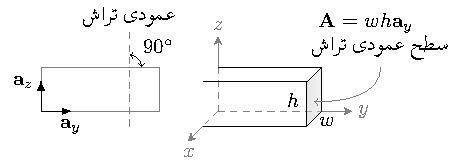
\includegraphics[height=2.5cm]{figBasicFactsCrossSectionalArea}
\caption{رقبہ  عمودی تراش}
\label{شکل_حقائق_رقبہ_عمودی}
\end{figure}
%
\حصہ{برقی اور مقناطیسی میدان}
\جزوحصہ{برقی میدان اور برقی میدان کی شدت}
\اصطلاح{کولمب کے قانون}\فرہنگ{قانون!کولمب}\حاشیہب{Coulomb's law}\فرہنگ{Coulomb's law} کے تحت \اصطلاح{برقی بار}\فرہنگ{برقی بار}\حاشیہب{electric charge}\فرہنگ{charge} سے لدے جسموں کے درمیان قوت کشش\حاشیہب{attractive force} یا قوت دفع\حاشیہب{repulsive force} ان اجسام پر \اصطلاح{بار}\حاشیہب{charge}  کے حاصل ضرب کے راست متناسب اور باہمی فاصلہ کے مربع کے بالعکس متناسب ہوتی ہے۔ یوں بار \عددی{q_1} اور \عددی{q_2} جن کے درمیان فاصلہ \عددی{r} ہو کے بیچ قوت \عددی{F} درج ذیل ہو گا جہاں \عددی{\epsilon}\حاشیہب{electric constant, electric permittivity} برقی مستقل ہے۔ 
\begin{align}\label{مساوات_بنیادی_کولمب_کا_قانون}
F=\frac{q_1 q_2}{4 \pi \epsilon r^2}
\end{align}
ایک برقی بار کے قریب  دوسرا برقی بار لانے سے  (پہلے اور) دوسرے برقی بار پر کشش یا دفع کی قوت عمل کرے گی جس کا تعین قانون کولمب سے ہوتا ہے۔ دوسرے برقی بار کو پہلے برقی بار سے آہستہ آہستہ دور کرنے سے  قوت کشش یا دفع بتدریج کم ہوتی ہے جو ایک خاص فاصلے کے بعد تقریباً صفر ہو جاتی ہے اور دوسرا بار پہلے بار کے حلقہ اثر سے باہر ہو جاتا ہے۔ یہ حلقہ   \اصطلاح{برقی میدان}\فرہنگ{برقی میدان} کہلاتا ہے۔ برقی میدان کسی ایک بار یا متعدد  باروں کی وجہ سے ہو سکتا ہے۔ 

\ابتدا{تعریف}
 کسی بار کے برقی میدان سے مراد بار کے اِردگرد وہ حلقہ ہے جس میں اس کا برقی اثر محسوس کیا جاتا ہے-
\انتہا{تعریف}

برقی میدان میں اکائی مثبت بار پر قوت اس مقام پر  \اصطلاح{برقی میدان کی شدت}\فرہنگ{برقی میدان!شدت}\حاشیہب{electric field intensity}\فرہنگ{electric field!intensity} (\سمتیہ{E} کی مطلق قیمت) دیگا جبکہ اکائی بار پر قوت کا رخ برقی میدان کا رخ دیگا۔برقی میدان کی شدت کی اکائی \اصطلاح{وولٹ فی میٹر}\حاشیہب{\si{\volt / \meter}} ہے۔

قانون کولمب (مساوات \حوالہ{مساوات_بنیادی_کولمب_کا_قانون})   سے   \عددیء{Q} بار کے برقی میدان کی شدت کی مطلق قی ت حاصل کرتے  ہیں۔بار  \عددیء{Q} اور اکائی بار (ایک کولمب بار) کے بیچ  قوتِ کشش یا قوتِ دفع 
\begin{align}
F=\frac{Q \times 1}{4 \pi \epsilon r^2}=\frac{Q}{4\pi\epsilon r^2}
\end{align}
نیوٹن ہو گی۔یہی برقی میدان کی شدت کی مطلق قیمت ہو گی:
\begin{align}
E=\frac{Q}{4\pi\epsilon r^2}
\end{align}
دو باروں  کے مابین قوتِ کشش یا قوتِ دفع کا رخ ان کے درمیان کھینچی گئی سیدھی لکیر پر ہو گا۔

\جزوحصہ{مقناطیسی میدان اور مقناطیسی میدان کی شدت}
\اصطلاح{مقناطیسی میدان} اور \اصطلاح{مقناطیسی میدان کی شدت}\فرہنگ{مقناطیسی میدان!شدت}\حاشیہب{magnetic field intensity}\فرہنگ{magnetic field!intensity} بالترتیب بالکل برقی میدان اور برقی میدان کی شدت کی طرح ہیں۔


\ابتدا{تعریف}
کسی مقناطیس کے مقناطیسی میدان سے مراد مقناطیس کے اِردگرد وہ حلقہ ہے جس میں اس کا مقناطیسی اثر محسوس کیا جاتا ہو۔
\انتہا{تعریف}


\حصہ{سطحی اور حجمی  کثافت}
\جزوحصہ{سطحی کثافت}
اکائی رقبہ کی سطح پر کسی چیز کی کل مقدار کو اس چیز کی \اصطلاح{سطحی کثافت}\فرہنگ{سطحی کثافت}\حاشیہب{surface density}\فرہنگ{surface density} کہتے ہیں۔ یوں رقبہ \عددیء{A} پر کسی چیز کی کل مقدار  \عددیء{\phi} ہونے کی صورت میں اس  کی اوسط سطحی کثافت \سیدھازیرنوشت{B}{اوسط}   درج ذیل ہو گی۔
\begin{align}
B_{\textup{اوسط}}=\frac{\phi}{A}
\end{align}
اس مساوات سے 
\begin{align}
\phi=B_{\textup{اوسط}} A
\end{align}
لکھا جا سکتا ہے جو کسی سطح پر ایک متغیرہ کی اوسط سطحی کثافت معلوم ہونے کی صورت میں  سطح پر متغیرہ کی کل مقدار دیتی ہے۔

غیر یکساں  متغیرہ کی صورت میں سطحی کثافت جگہ جگہ مختلف ہو گی۔ ایسی صورت میں  اتنے چھوٹے رقبے پر، جس میں متغیرہ کو 
یکساں تصور کیا جا سکتا ہو، سطحی کثافت
\begin{align}
B=\frac{\Delta \phi}{\Delta A}
\end{align}
ہو گی جہاں \عددیء{\Delta A} چھوٹا رقبہ اور  \عددیء{\Delta \phi} اس رقبے  پر متغیرہ کی چھوٹی مقدار ہے۔ اس چھوٹے رقبہ کو نقطہ مانند کرنے سے  نقطی کثافت 
\begin{align}
B=\frac{\dif \phi}{\dif A}
\end{align}
 حاصل ہو گی جس کو 
\begin{align}
\dif \phi =B \dif A
\end{align}
بھی لکھا  جا سکتا ہے۔  یوں نقطی کثافت جانتے ہوئے  ایک نقطہ کے  چھوٹے  رقبہ پر  متغیرہ کی  کل (چھوٹی) مقدار معلوم کی جا سکتی ہے۔

یوں  ایک برقی تار جس کا رقبہ عمودی تراش \عددیء{A}  اور جس میں برقی رو \عددیء{I}  کی  اوسط کثافتِ برقی رو  درج ذیل ہو گی۔
\begin{align}\label{مساوات_بنیادی_برقی_رو_کثافت}
\rho_{\textup{اوسط}}=\frac{I}{A}
\end{align}

\حصہ{حجمی کثافت}
  اکائی حجم میں کسی چیز کی کل مقدار کو اس چیز کی \اصطلاح{حجمی کثافت} کہتے ہیں۔یوں اگر کسی چیز کا حجم \عددیء{H} اور اس کی کمیت \عددیء{m} ہو تب اس کی اوسط (کمیتی) حجمی کثافت درج ذیل  ہو گی۔
\begin{align}
\rho_{\textup{اوسط}}=\frac{m}{H}
\end{align}
غیر یکساں کمیت کی صورت میں  حجم میں مختلف مقامات پر  کمیت مختلف ہو گا۔ ایسی  صورت میں اتنا چھوٹا حجم لیتے ہوئے  جس میں کمیت کو  یکساں تصور کیا جا سکتا ہو،  حجمی کثافت درج ذیل ہو گی۔
\begin{align}
\rho=\frac{\Delta m}{\Delta H}
\end{align}
اس چھوٹے حجم  کو نقطہ مانند بنانے سے درج ذیل  نقطی حجمی کثافت لکھی جا سکتی ہے۔
\begin{align}
\rho=\frac{\dif m}{\dif H}
\end{align}
یوں 
\begin{align}
\dif m=\rho \dif H
\end{align}
ہو گا لہٰذا  نقطی حجمی کثافت جانتے ہوئے ایک چھوٹے حجم کی (چھوٹی) کمیت حاصل کی جا  سکتی ہے۔

\حصہ{صلیبی ضرب اور ضرب نقطہ}
دو غیر سمتی متغیرات کا حاصل ضرب غیر سمتی متغیر ہوتا ہے جبکہ دو سمتیات  کا حاصل ضرب سمتی  یا غیر سمتی ہو سکتا ہے۔ان دو اقسام کے ضرب پر یہاں غور کیا جائے گا۔

\جزوحصہ{صلیبی ضرب}
دو سمتی متغیرات  کا ایسا ضرب جو سمتی متغیر دیتا ہو  \اصطلاح{صلیبی ضرب}\فرہنگ{ضرب صلیبی}\حاشیہب{cross product}\فرہنگ{cross product} کہلاتا اور درج ذیل لکھا جاتا ہے۔
\begin{align}
\kvec{C}=\kvec{A} \times \kvec{B}
\end{align}
صلیبی ضرب میں ضرب کے نشان کو صلیب کی علامت سے ظاہر کیا جاتا ہے جس کی بنا اس کو صلیبی ضرب کہتے ہیں۔

حاصل ضرب سمتیہ \سمتیہ{C} کی مقدار
\begin{gather}
\begin{aligned}\label{مساوات_بنیادی_ضرب_صلیبی_تعریف}
C=\abs{\kvec{C}} &= \abs {\kvec{A}} \abs{\kvec{B}} \sin \theta_{AB}\\
&=A B \sin \theta_{AB}
\end{aligned}
\end{gather}
ہے جہاں \عددیء{\theta_{AB}} ان کے مابین زاویہ ہے۔اس حاصل سمتیہ کی سمت دائیں ہاتھ  کے قانون سے  حاصل کی جاتی ہے۔ یوں دائیں ہاتھ کا انگوٹھا، شہادت کی انگلی اور  بڑی انگلی کو ایک دوسرے کے ساتھ \عددی{90^{\circ}} زاویہ پر رکھتے ہوئے، شہادت کی انگلی کو سمتیہ{A} اور بڑی انگلی کو \سمتیہ{B}  کے رخ رکھنے سے  انگوٹھا \سمتیہ{C} کا رخ دیگا۔


\ابتدا{مثال}
درج ذیل ضرب صلیبی حاصل کریں۔
\begin{itemize}
\item
$\ax \times \ay \quad \ay \times \az \quad \az \times \ax \quad \ax \times \az$ 
\item
 $\az \times \ay \quad \ay \times \ay \quad \arho \times \atheta \quad \az \times \arho$
\end{itemize}

حل: اس مثال میں سب سمتیات اکائی ہیں۔اکائی سمتیہ کا طول ایک کے برابر ہوتا ہے لہٰذا درج ذیل ہوں گے۔
\begin{itemize}
\item
$\ax \times \ay=(1)(1) \sin 90 \az =\az$
\item
$\ay \times \az=(1)(1) \sin 90 \ax =\ax$
\item
$\az \times \ax=(1)(1) \sin 90 \ay =\ay$
\item
$\ax \times \az=(1)(1) \sin 90 (-\ay) =-\ay$
\item
$\az \times \ay=(1)(1) \sin 90 (-\ax) =-\ax$
\item
چونکہ دونوں سمتیات کے رخ ایک جیسے ہیں لہٰذا ان کے مابین زاویہ صفر ہو گا۔صفر زاویہ کا سائن بھی صفر ہوتا ہے، \عددیء{\sin 0 =0}۔ یوں ان دو سمتیات  کا ضرب صلیبی صفر ہو گا۔\\
$\ay \times \ay=(1)(1) \sin 0  =0$
\item
$\arho \times \atheta=(1)(1) \sin 90  \az =\az$
\item
$\az \times \arho=(1)(1) \sin 90 \atheta =\atheta $
\end{itemize}
\انتہا{مثال}
%
\ابتدا{مثال}
شکل \حوالہ{شکل_حقائق_کارتیسی_مروڑ_کا_حل} میں  چار نیوٹن کی قوت \سمتیہ{F} محور سے تین میٹر کی سمتی فاصلہ \سمتیہ{L}  پر لاگو ہے جس  کی تفصیل شکل میں دی گئی ہے۔اس قوت کی قوت مروڑ  حاصل کریں۔
حل:	قوت مروڑ \سمتیہ{T} کی تعریف درج ذیل  ہے۔
\begin{align}
\kvec{T}=\kvec{L} \times \kvec{F}
\end{align}
کارتیسی نظام میں یہ سمتی فاصلہ
\begin{align}
\kvec{L}=L \sin \theta \ax-L \cos \theta \ay
\end{align}
ہو گا لہٰذا
\begin{align*}
\kvec{T}&=\left(L \sin \theta \ax-L \cos \theta \ay \right) \times F \ay\\
&=L \sin \theta \ax \times F \ay-L \cos \theta \ay \times F \ay\\
&= L F \sin \theta \az
\end{align*} 
ہو گا جہاں پچھلی مثال کی مدد سے \عددیء{\ax \times \ay=\az} اور \عددیء{\ay \times \ay=0} لئے گئے ہیں۔یوں درج ذیل ہو گا۔
\begin{align*}
\kvec{T}= L F \sin \theta \az=12 \sin \theta \az \quad \si{\newton \meter}
\end{align*}
اس مثال میں \عددیء{\theta_{LF}=180\degree-\theta} ہے۔چونکہ کسی بھی زاویہ \عددیء{\alpha}   کے لئے \عددیء{\sin \alpha=\sin(180\degree-\alpha)} ہوتا ہے لہٰذا اس قوت مروڑ کو درج ذیل بھی لکھا جا سکتا ہے۔
\begin{align*}
\kvec{T}&=LF\sin \theta \az\\
&=L F \sin \theta_{LF}\az
\end{align*}
یہی جواب ضرب صلیبی کی تعریف یعنی مساوات \حوالہ{مساوات_بنیادی_ضرب_صلیبی_تعریف} اور دائیں ہاتھ کے قانون کی مدد سے زیادہ آسانی سے حاصل ہوتا ہے۔
\انتہا{مثال}
%
\begin{figure}
\centering
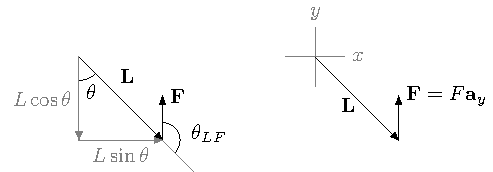
\includegraphics[height=2.5cm]{figBasicFactsVectorCrossProduct}
\caption{کارتیسی نظام میں قوت مروڑ کا حل}
\label{شکل_حقائق_کارتیسی_مروڑ_کا_حل}
\end{figure}
%
\جزوحصہ{نقطی ضرب}
دو سمتی متغیرات  کا ایسا حاصل ضرب جو غیر سمتی متغیر ہو \اصطلاح{نقطی ضرب}\فرہنگ{ضرب!نقطہ}\حاشیہب{dot product}\فرہنگ{dot product} کہلاتا ہے جو درج ذیل لکھا جاتا ہے۔
\begin{align}
\kvec{C}=\kvec{A} \cdot \kvec{B}
\end{align}
نقطی ضرب میں ضرب کے نشان کو نقطہ کی علامت سے ظاہر کیا جاتا ہے جس کی بنا پر اس کا نام نقطی ضرب ہے۔

نقطی ضرب کی مقدار  درج ذیل ہو گی
\begin{gather}
\begin{aligned}\label{مساوات_بنیادی_ضرب_نقطہ_تعریف}
\kvec{C}&=\kvec{A} \cdot \kvec{B}\\
&=\abs{\kvec{A}} \abs{\kvec{B}} \cos \theta_{AB}\\
&=A B \cos \theta_{AB}
\end{aligned}
\end{gather}
جہاں \عددیء{\theta_{AB}} ان سمتیات کے بیچ زاویہ ہے۔

\ابتدا{مثال}
مندرجہ ذیل نقطی ضرب حاصل کریں۔
\begin{itemize}
\item
$\ax \cdot \ax \quad \ay \cdot \ay \quad \az \cdot \az$
\item
$\ax \cdot \ay \quad \ay \cdot \az \quad \arho \cdot \arho \quad \arho \cdot \atheta$
\end{itemize}

حل:اس مثال میں سب سمتیات اکائی  ہیں۔اکائی سمتیہ کا طول ایک (1) کے برابر ہوتا ہے:
\begin{itemize}
\item
$\ax \cdot \ax =(1) (1) \cos 0=1$
\item
$\ay \cdot \ay =(1) (1) \cos 0=1$
\item
$\az \cdot \az =(1) (1) \cos 0=1$
\item
$\ax \cdot \ay =(1) (1) \cos 90\degree=0$
\item
$\ay \cdot \az =(1) (1) \cos 90\degree=0$
\item
$\arho \cdot \arho =(1) (1) \cos 0=1$
\item
$\arho \cdot \atheta =(1) (1) \cos 90\degree=0$
\end{itemize}
\انتہا{مثال}
%=========================
\ابتدا{مثال}
شکل \حوالہ{شکل_حقائق_کارتیسی_کام}  میں قوت \سمتیہ{F} ایک بوجھ کو دھکیل رہی ہے۔سمتی فاصلہ  \سمتیہ{L} طے کرنے پر قوت کتنا کام کر چکی ہو گی۔

حل: کام  \عددیء{W} کی تعریف درج ذیل  ہے۔
\begin{align}
W=\kvec{F} \cdot \kvec{L}
\end{align}
کارتیسی نظام میں سمتی فاصلہ 
\begin{align}
\kvec{L}=L \cos \theta \ax +L \sin \theta \ay
\end{align}
ہو گا۔ یوں درج ذیل ہو گا
\begin{gather}
\begin{aligned}
W &= (F \ax) \cdot (L \cos \theta \ax +L \sin \theta \ay)\\
&=F L \cos \theta (\ax \cdot \ax)+ F L \sin \theta (\ax \cdot \ay)\\
&= F L \cos \theta
\end{aligned}
\end{gather}
%
\begin{figure}
\centering
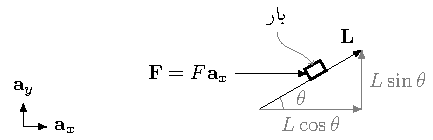
\includegraphics[height=2.5cm]{figBasicFactsWorkAsDotProduct}
\caption{کارتیسی نظام میں کام}
\label{شکل_حقائق_کارتیسی_کام}
\end{figure}
جہاں پچھلی مثال کی مدد سے \عددیء{\ax \cdot \ax=1} اور \عددیء{\ax \cdot \ay=0} لیے گئے ہیں۔ یہی جواب نقطی ضرب کی تعریف، مساوات \حوالہ{مساوات_بنیادی_ضرب_نقطہ_تعریف}،  سے با آسانی حاصل ہوتا ہے۔
\انتہا{مثال}
%
\حصہ{تفرق  اور جزوی تفرق}
مساوات \حوالہ{مساوات_بنیادی_تفرق} میں ایک تفاعل  کا \اصطلاح{تفرق}\فرہنگ{تفرق}\حاشیہب{differentiation}\فرہنگ{differentiation} دیا گیا ہے، جس میں \عددیء{B_0} ایک مستقل ہے، جبکہ مساوات \حوالہ{مساوات_بنیادی_جزوی_تفرق}  میں ایک تفاعل کا \اصطلاح{جزوی تفرق}\فرہنگ{تفرق!جزوی}\حاشیہب{partial differentiation}  دیا گیا ہے۔
\begin{gather}
\begin{aligned}\label{مساوات_بنیادی_تفرق}
B (\theta )&=B_0 \cos \theta\\
\frac{\dif B}{\dif \theta}&=-B_0 \sin \theta
\end{aligned}
\end{gather} 
%
\begin{align}\label{مساوات_بنیادی_جزوی_تفرق}
\partial W(x,\lambda)=\frac{\partial W}{\partial x} \dif x+\frac{\partial W}{\partial \lambda} \dif \lambda
\end{align}

%%%%%%%%%%%%%%%%%%%%%%%

\حصہ{خطی تکمل}
مساوات \حوالہ{مساوات_بنیادی_سائن_نما_تفاعل}  میں ایک تفاعل \عددیء{B(\theta)} دیا گیا ہے جسے شکل \حوالہ{شکل_حقائق_کوسائن_موج}  میں دکھایا گیا ہے۔ اس کی \اصطلاح{طولِ موج}\فرہنگ{طول موج}\حاشیہب{wavelength}  \عددیء{2 \pi} ریڈیئن کے برابر ہے۔ ہم \عددیء{-\pi/2<\theta<\pi/2} کے مابین اس کا اوسط معلوم کرتے ہیں۔ یہ \اصطلاح{تکمل}\فرہنگ{تکمل}\حاشیہب{integration} سے یوں ہو گا۔
\begin{align}\label{مساوات_بنیادی_سائن_نما_تفاعل}
B(\theta)=B_0 \cos \theta
\end{align}
%
\begin{align}
B_{\textup{اوسط}}=\frac{B_0}{\pi}\int_{-\frac{\pi}{2}}^{\frac{\pi}{2}} \cos \theta \dif \theta=\frac{2 B_0}{\pi}
\end{align}
اسی طرح اگر اسی خطہ پر تفاعل کے مربع یعنی \عددیء{B^2}  کا اوسط درکار ہو تو ایسا کرنا مساوات \حوالہ{مساوات_بنیادی_سائن_نما_اوسط_مربع} میں دکھایا گیا ہے۔
\begin{gather}
\begin{aligned}\label{مساوات_بنیادی_سائن_نما_اوسط_مربع}
B^2_{\textup{اوسط}}&=\frac{B_0^2}{\pi}\int_{-\frac{\pi}{2}}^{\frac{\pi}{2}} \cos^2 \theta \dif \theta\\
&=\frac{B_0^2}{\pi}\int_{-\frac{\pi}{2}}^{\frac{\pi}{2}}\frac{1+\cos 2 \theta}{2} \dif \theta\\
&=\frac{B_0^2}{2}
\end{aligned}
\end{gather}
تفاعل کے مربع کی اوسط کا جزر  بہت اہمیت رکھتا ہے۔لہٰذا اس تفاعل کے مربع کی اوسط کا جزر \عددیء{B_{\textup{موثر}}} مساوات \حوالہ{مساوات_بنیادی_سائن_نما_اوسط_مربع}  کی مدد سے یوں حاصل ہوتا ہے۔
\begin{align}\label{مساوات_بنیادی_سائن_نما_کی_موثر_قیمت}
B_{\textup{موثر}}=\sqrt{B^2_{\textup{اوسط}}}=\frac{B_0}{\sqrt{2}}
\end{align}
یہ ایک بہت اہم نتیجہ ہے جو آپ کو زبانی یاد ہونا چاہئے۔ یہ مساوات ہر سائن نما تفاعل کے لئے درست ہے۔کسی بھی متغیرہ کے مربع کی اوسط کا جزر اس متغیرہ کی \اصطلاح{موثر}\فرہنگ{موثر}\حاشیہب{effective}\حاشیہب{root mean square, rms} قیمت کہلاتا ہے۔
%
\begin{figure}
\centering
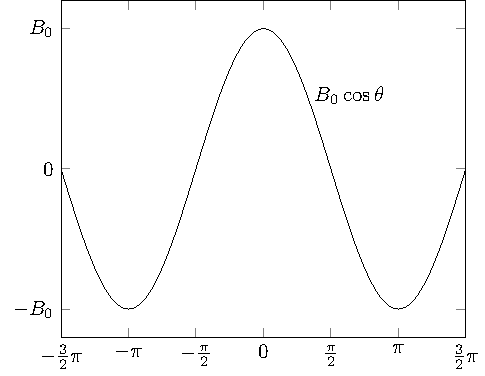
\includegraphics{figBasicFactsCosineWave}
\caption{کوسائن موج}
\label{شکل_حقائق_کوسائن_موج}
\end{figure}
\حصہ{سطحی تکمل}
مثال کے طور پر اگر مساوات \حوالہ{مساوات_بنیادی_سائن_نما_تفاعل}  شکل  \حوالہ{شکل_حقائق_نلکی_سطحی_تکمل} میں نلکی کے بیرونی سطح پر متغیرہ \عددیء{B} کی مقدار بتلاتی ہے اور یہ متغیرہ سطحی کثافت کو ظاہر کرے  ہم آدھے بیرونی سطح مثلاً زاویہ \عددیء{-\pi/2} اور \عددیء{\pi/2} کے مابین اس کی کل مقدار \عددیء{\phi} معلوم کرتے ہیں۔اس سطح میں نلکی کے دونوں سرے شامل نہیں ہیں۔

	ہم نلکی کے بیرونی سطح پر رقبہ  \عددیء{\Delta A} لیتے ہیں جس کی چوڑائی \عددیء{\rho \Delta\theta}  اور لمبائی \عددیء{l} ہے۔یہ سطح \عددیء{abcd} ہے۔\عددیء{\Delta \theta} کو نہایت کم کرتے ہوئے سطح کا رقبہ \عددیء{\rho l \dif \theta} لکھا جا سکتا ہے۔اس سطح پر \عددیء{B} کی مقدار محوری لمبائی  کی جانب تبدیل نہیں ہو رہی۔سطح \عددیء{\Delta A}  پر \عددیء{\Delta \phi=B \Delta A} ہو گا اور کل \عددیء{\phi} تکمل کی مدد سے یوں حاصل ہو گا۔
\begin{figure}
\centering
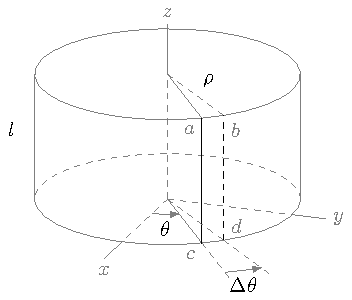
\includegraphics{figBasicFactsCylindricalSurfaceIntegral}
\caption{نلکی کی بیرونی سطح پر متغیرہ کا تکمل کل مقدار دے گی۔}
\label{شکل_حقائق_نلکی_سطحی_تکمل}
\end{figure}
%
\begin{align}
\Delta \phi=B \Delta A=B_0 l \rho \cos \theta \dif \theta
\end{align}
%
\begin{align}\label{مساوات_بنیادی_بہاو_بذریع_تکمل_زاویہ_صفر}
\phi = B_0 l \rho \int_{-\pi/2}^{\pi/2} \cos \theta \dif \theta =2 B_0 l \rho
\end{align}
اب ہم یہی مقدار نلکی کے آدھے بیرونی سطح پر کہیں پر بھی حاصل کرنا چاہیں تو ہمیں صرف تکمل کے دو حد تبدیل کرنے ہوں گے۔  اگر ہم مساوات \حوالہ{مساوات_بنیادی_بہاو_بذریع_تکمل_زاویہ_صفر}  میں نچلا حد \عددیء{(-\pi/2-\alpha)} اور اوپر کا حد \عددیء{(\pi/2-\alpha)} لیں تو یہ حاصل ہو گا۔
\begin{align}\label{مساوات_بنیادی_بہاو_بذریع_تکمل_کوئی_زاویہ}
\phi (\alpha) = B_0 l \rho \int_{-\frac{\pi}{2}-\alpha}^{\frac{\pi}{2}-\alpha} \cos \theta \dif \theta =2 B_0 l \rho \cos \alpha
\end{align}
یہاں  \عددیء{\phi(\alpha)} اس بات کو واضح کرتا ہے کہ نتیجہ \عددیء{\alpha} پر منحصر ہے۔ یہ ایک بہت اہم مساوات ہے۔ مساوات \حوالہ{مساوات_بنیادی_بہاو_بذریع_تکمل_کوئی_زاویہ} میں  اگر \عددیء{\alpha=0} ہو تو مساوات \حوالہ{مساوات_بنیادی_بہاو_بذریع_تکمل_زاویہ_صفر}   ملتا ہے۔

\حصہ{ مرحلی سمتیہ}
\begin{figure}
\centering
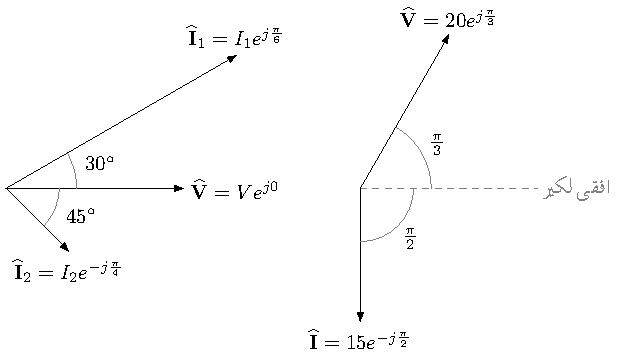
\includegraphics{figBasicFactsPhasors}
\caption{مرحلی سمتیہ}
\label{شکل_حقائق_دوری_سمتیات}
\end{figure}
سائن نما موج جن کا تعدد معین ہو کو مرحلی سمتیہ سے ظاہر کرنا نہایت مفید ثابت ہوتا ہے۔ مساوات \اصطلاح{یولر}\فرہنگ{یولر مساوات}\حاشیہب{Euler's equation}\فرہنگ{Euler}
\begin{align}
A_0 e^{\mp j (\omega t + \phi)}=A_0 \cos (\omega t +\phi) \mp j \sin (\omega t+\phi)
\end{align}
کی مدد سے کوسائن موج یوں لکھی جا سکتی ہے
\begin{align}
A_0 \cos (\omega t +\phi)=\frac{A_0}{2} \left(e^{j(\omega t +\phi)} -e^{-j(\omega t +\phi)}\right)
\end{align}
اس سے ثابت ہوتا ہے کہ کوسائن موج دراصل دو مخلوط اعداد کا مجموعہ ہے۔ مساوات یولر ایک مخلوط عدد کو ظاہر کرتا ہے جس کے دو جزو ہیں۔ اس کا ایک جزو حقیقی عدد ہے اور اس کا دوسرا جزو فرضی عدد ہے۔اس کا حقیقی جزو کوسائن موج کو ظاہر کرتا ہے۔ لہٰذا ایک کوسائن موج  \عددیء{A_0 e^{j(\omega t +\phi)}} یا \عددیء{A_0 e^{-j(\omega t +\phi)}} کا حقیقی جزو ہوتا ہے۔ رسمی طور پر سائن نما موج کو \عددیء{A_0 e^{j(\omega t +\phi)}} سے ظاہر کیا جاتا ہے۔ مزید یہ کہ اس عدد کو چھوٹا کر کے صرف \عددیء{A_0 e^{j\phi}} یا پھر \عددیء{A_0 \phase{\phi}} لکھا جاتا ہے۔کوسائن موج کے اس طرح ظاہر کرنے کو \اصطلاح{مرحلی سمتیہ}\فرہنگ{مرحلی سمتیہ}\حاشیہب{phasor}\فرہنگ{phasor} کہتے ہیں جہاں اس سمتیہ کا طول \عددیء{A_0} اور افقی لکیر سے زاویہ \عددیء{\phi} ہے۔

	 مرحلی سمتیہ استعمال کرتے وقت آپ کو یہ ذہن میں رکھنا ہوتا ہے کہ یہ ایک کوسائن موج ہے جس کا حیطہ  \عددیء{A_0} ، دوری زاویہ \عددیء{\phi} اور زاویائی تعدد \عددیء{\omega} ہے۔

اس کتاب میں مرحلی سمتیہ کو سادہ طرزِ لکھائی میں انگریزی کے بڑے حروف جن پر ٹوپی کا نشان ہو سے ظاہر کیا جائے گا، یعنی \عددیء{\hat{I},\hat{V}}  وغیرہ اور ان کے طول کو بغیر ٹوپی کے نشان کے اسی حرف سے ظاہر کیا جائے گا۔مثلاً برقی دباو \عددیء{v= 20 \cos (\omega t +\frac{\pi}{3})} کے لئے یہ سب درست ہیں۔
\begin{gather}
\begin{aligned}
v&=20 \cos (\omega t +\frac{\pi}{3})\\
\hat{V}&=20 e^{j \frac{\pi}{3}}\\
\hat{V}&=20 \phase{\frac{\pi}{3}}\\
V&=20
\end{aligned}
\end{gather}
اس مساوات میں پہلا جزو ایک عام کوسائن موج ہے۔ دوسرا جزو اِسی کو مرحلی سمتیہ سے ظاہر کر رہا ہے۔ تیسرا اس مرحلی سمتیہ کا طول اور چوتھا اس کا زاویہ بتلا رہا ہے۔
\begin{figure}
\centering
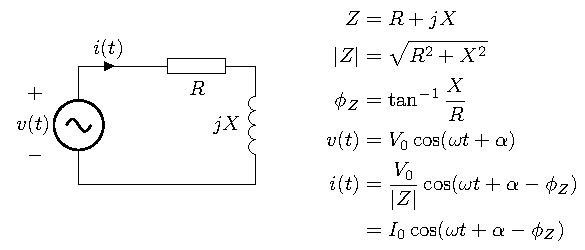
\includegraphics{figBasicFactsRLcircuit}
\caption{مرحلی سمتیہ کی مدد سے \عددیء{RL} دور کا حل۔}
\label{شکل_حقائق_دوری_سمتیہ_سے_دور_حل}
\end{figure}
	مرحلی سمتیہ کو عام سمتیوں کی طرح ہی تصور کیا جاتا ہے۔ اس مساوات میں \عددیء{\hat{V}} کا طول \عددیء{20} اور افقی لکیر سے زاویہ  \عددیء{\tfrac{\pi}{3}} ریڈیئن ہے۔زاویہ افقی لکیر سے گھڑی کی الٹی سمت ناپا جاتا ہے۔ اس سمت میں زاویہ مثبت ہے۔ شکل \حوالہ{شکل_حقائق_دوری_سمتیات} میں اس \عددیء{\hat{V}} کے علاوہ چند اور مرحلی سمتیے دکھائے گئے ہیں۔

برقی ادوار میں عموماً برقی دباو \عددیء{\hat{V}} کی نسبت سے  برقی رو  \عددیء{\hat{I}} کا زاویہ بیان کیا جاتا ہے۔شکل \حوالہ{شکل_حقائق_دوری_سمتیات}   میں \عددیء{\hat{I_1}} تیس درجہ زاویہ برقی دباو سے آگے ہے جبکہ  \عددیء{\hat{I_2}}  پینتالیس درجہ زاویہ برقی دباو کے  پیچھے  ہے۔اس حقیقت کو یوں بیان کیا جاتا ہے کہ \عددیء{\hat{I_1}} تیس درجہ  \اصطلاح{پیش زاویہ}\فرہنگ{پیش زاویہ}\حاشیہب{leading angle}\فرہنگ{leading} پر  ہے جبکہ  \عددیء{\hat{I_2}} پینتالیس درجہ  \اصطلاح{تاخیری زاویہ}\فرہنگ{تاخیری زاویہ}\حاشیہب{lagging angle}\فرہنگ{lagging} پر ہے۔اسے طرح \عددیء{\hat{I_1}} کو \اصطلاح{پیش} برقی رو جبکہ \عددیء{\hat{I_2}} کو \اصطلاح{تاخیری} برقی رو کہا جاتا ہے۔دو مرحلی سمتیات کے آپس میں زاویے کو \اصطلاح{مرحلی فرق}\فرہنگ{مرحلی فرق}\حاشیہب{phase difference}\فرہنگ{phase difference} کہتے ہیں لہٰذا \عددیء{\hat{I_1}} اور \عددیء{\hat{I_2}} میں \عددیء{75 \degree} کا مرحلی فرق پایا جاتا ہے۔یہاں یہ دھیان رہے کہ شکل میں  \عددیء{45\degree} مثبت لکھا گیا ہے۔چونکہ یہ افقی لکیر سے زاویہ ناپنے کی الٹ سمت میں ہے لہٰذا یہ ایک منفی زاویہ ہے۔

اگر \عددیء{v=V_0 \cos \omega t} اور \عددیء{i=I_0 \cos (\omega t +\theta)} ہوں تب برقی طاقت \عددیء{p=V_0 I_0 \cos \theta} کے برابر ہو گا جہاں \عددیء{\cos \theta} کو \اصطلاح{جزو طاقت}\فرہنگ{جزو طاقت}\حاشیہب{power factor}\فرہنگ{power factor}  اور \عددیء{\theta} کو \اصطلاح{زاویہ جزو طاقت}\فرہنگ{زاویہ جزو طاقت}\حاشیہب{power factor angle}\فرہنگ{power factor angle} کہتے ہیں۔ اسی طرح \اصطلاح{تاخیری} زاویہ کی صورت میں \عددیء{\cos \theta} کو \اصطلاح{تاخیری جزو طاقت}\فرہنگ{جزو طاقت!تاخیری}\حاشیہب{lagging power factor}\فرہنگ{power factor!lagging} اور \اصطلاح{پیش} زاویہ کی صورت میں \عددیء{\cos \theta} کو \اصطلاح{پیش جزو طاقت}\فرہنگ{جزو طاقت!پیش}\حاشیہب{leading power factor}\فرہنگ{power factor!leading} کہتے ہیں۔

یہاں مرحلی سمتیوں کو استعمال کر کے ایک سادہ برقی دور حل کرتے ہیں۔ یوں ان سے وابستگی پیدا ہو جائے گی اور ان کا استعمال بھی سیکھ لیں گے۔

شکل \حوالہ{شکل_حقائق_دوری_سمتیہ_سے_دور_حل}   ایک سادہ \عددیء{R-L} \اصطلاح{یک مرحلہ}\فرہنگ{یک مرحلہ}\حاشیہب{single phase}\فرہنگ{single phase} برقی دور ہے جس پر لاگو برقی دباو
\begin{gather}
\begin{aligned}
v(t)&=V_0 \cos (\omega t +\alpha)\\
\hat{V}&=V_0 \phase{\alpha}
\end{aligned}
\end{gather}
ہے۔مرحلی سمتیہ کے استعمال سے ہم اس میں برقی رو \عددیء{i(t)} معلوم کرنا چاہتے ہیں۔
\begin{gather}
\begin{aligned}
\hat{I}&=\frac{\hat{V}}{R+j X}=\frac{V_0 \phase{\alpha}}{\abs{Z} \phase {\phi_Z}}\\
&=\frac{V_0}{\abs{Z}} \phase{\alpha-\phi_Z}=I_0 \phase{\alpha-\phi_Z}
\end{aligned}
\end{gather}
جہاں \عددیء{\phi_Z} رکاوٹ کا زاویہ  ہے۔لہٰذا
\begin{align}\label{مساوات_بنیادی_حقائق_دوری_سمتیہ_سے_مزاحمت_امالہ_دور_حل}
i(t)=I_0 \cos (\omega t +\alpha-\phi_Z)
\end{align}
حاصل ہوتا ہے۔یوں \اصطلاح{تاخیری} زاویہ \عددیء{\phi_Z} کے برابر ہے۔
